\section{Resultados}\label{sec:resultados}

\subsection{Treino e desempenho do classificador}
O F1-macro na validação estabilizou-se a partir da época 20, enquanto a perda no treino continuou caindo (Fig.~\ref{fig:treino}); o melhor modelo foi o da época 36, e o treino parou na época 46. Com a entropia cruzada ponderada, o F1-macro no teste foi de 0,816, contra 0,819 sem ponderação, uma diferença menor que a variação de cerca de 0,01 entre dois treinos anteriores com a mesma perda ponderada; a versão sem ponderação, que segue a referência, foi mantida. Os limiares escolhidos na validação foram: SNR 0,89; AF 0,58; IAVB 0,99; BRE 0,85; BRD 0,36; CAP 0,55; CVP 0,84; STD 0,34; STE 0,41. O F1 variou pouco numa faixa ampla de limiares em torno do escolhido (Fig.~\ref{fig:limiar}).

\begin{figure*}[!t]\centering
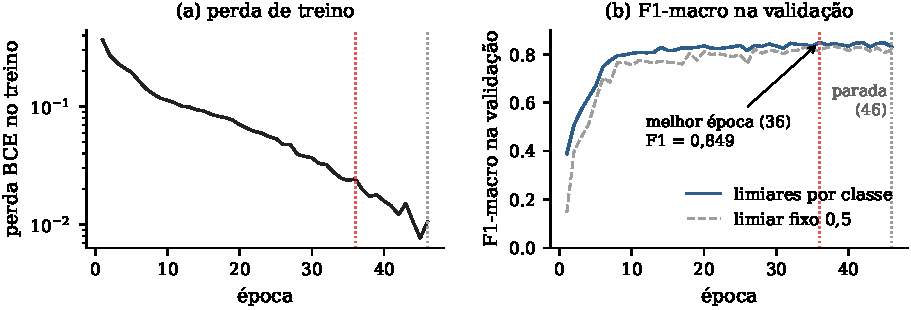
\includegraphics[width=0.66\textwidth]{figs/treino.pdf}
\caption{O F1 na validação estabiliza-se por volta da época 20, embora a perda no treino continue caindo, o que justificou a parada antecipada. (a) Perda no treino (escala logarítmica). (b) F1-macro na validação, com os limiares por classe e com o limiar fixo de 0,5. As linhas pontilhadas marcam a melhor época (36) e a parada (46).}\label{fig:treino}
\end{figure*}

\begin{figure}[!t]\centering
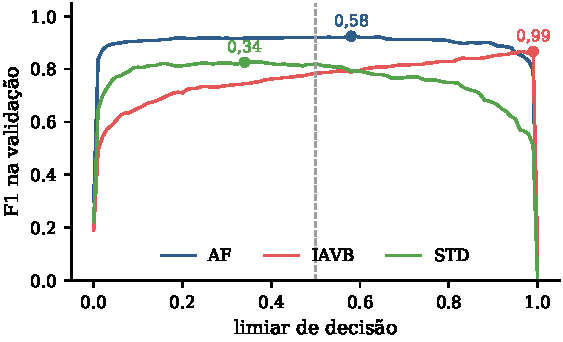
\includegraphics[width=\columnwidth]{figs/limiar.pdf}
\caption{O limiar de maior F1 é diferente em cada classe e, em várias delas, o F1 muda pouco numa faixa ampla de limiares. F1 na validação em função do limiar, para três classes; o ponto marca o limiar escolhido e a linha tracejada, o limiar de 0,5.}\label{fig:limiar}
\end{figure}

O modelo obteve F1-macro de 0,819 no teste, próximo do relatado por Zhang et al.\ na mesma base (0,813, média de 10 dobras)~\cite{zhang2021}. O F1 por classe também foi próximo do da referência (Tabela~\ref{tab:f1}): AF e BRD ficaram acima de 0,92, e STE foi a pior classe nos dois casos. Essa ordem das classes pelo F1 é a referência das comparações seguintes.

\begin{table*}[!t]\centering
\caption{O F1 por classe é próximo do relatado na referência, com AF e BRD no alto e STE em último. F1 por classe no teste, com os limiares por classe e com o limiar de 0,5; F1 de Zhang et al.~\cite{zhang2021} (média de 10 dobras); e número de mapas explicados (predições corretas). Classes ordenadas pelo F1 deste estudo.}\label{tab:f1}
\begin{tabular}{lrrrrrrrrr|r}
\toprule
& AF & BRD & IAVB & BRE & CVP & SNR & STD & CAP & STE & Macro \\
\midrule
F1 (limiares por classe) & 0,931 & 0,927 & 0,884 & 0,870 & 0,837 & 0,796 & 0,778 & 0,750 & 0,596 & 0,819 \\
F1 (limiar 0,5) & 0,931 & 0,921 & 0,811 & 0,857 & 0,814 & 0,772 & 0,778 & 0,750 & 0,622 & 0,806 \\
F1, Zhang et al.~\cite{zhang2021} & 0,919 & 0,926 & 0,864 & 0,866 & 0,851 & 0,805 & 0,814 & 0,735 & 0,535 & 0,813 \\
Mapas explicados & 108 & 172 & 61 & 20 & 59 & 78 & 65 & 45 & 14 & 622 \\
\bottomrule
\end{tabular}
\end{table*}

\subsection{Variação própria do GradientSHAP}
O piso médio foi de 0,18, de 0,13 em BRD e BRE a 0,25 em CAP (Tabela~\ref{tab:res}). Com 50 sorteios por mapa, ele era de 0,36.

\subsection{Métricas por classe}
A Tabela~\ref{tab:res} traz o valor de cada métrica por classe, e a Tabela~\ref{tab:ordens}, a ordem das classes em cada uma. Nenhuma métrica reproduziu exatamente a ordem do F1. As métricas se dividiram em dois grupos.

\begin{table*}[!t]\centering
\caption{As métricas de fidelidade e de robustez favorecem BRD e BRE, enquanto a \CS\ e o \RL\ acompanham o F1 nas pontas. Métricas por classe, com as classes na ordem do F1. FC: \FC\ ($|S| = 9$). FE: \FE. Max-S: \MS. N.º efet.: número efetivo de regiões (\CX). Cons.: \CS\ (entre parênteses, o valor ao acaso). RL: distância do \RL\ às classes ausentes. Setas: sentido melhor.}\label{tab:res}
\begin{tabular}{lrrrrrrrr}
\toprule
\textbf{Classe} & \textbf{F1} & \textbf{FC} $\uparrow$ & \textbf{FE} $\uparrow$ & \textbf{Max-S} $\downarrow$ & \textbf{Piso} & \textbf{N.º efet.} $\downarrow$ & \textbf{Cons.} $\uparrow$ & \textbf{RL} $\uparrow$ \\
\midrule
AF   & 0,931 & 0,544 & 0,515 & 0,056 & 0,19 & 22,9 & 0,457 (0,145) & 1,687 \\
BRD  & 0,927 & 0,746 & 0,784 & 0,029 & 0,13 & 22,2 & 0,723 (0,231) & 1,632 \\
IAVB & 0,884 & 0,647 & 0,553 & 0,041 & 0,18 & 23,0 & 0,424 (0,081) & 1,607 \\
BRE  & 0,870 & 0,651 & 0,698 & 0,033 & 0,13 & 26,2 & 0,335 (0,026) & 1,622 \\
CVP  & 0,837 & 0,618 & 0,659 & 0,047 & 0,17 & 25,0 & 0,382 (0,078) & 1,626 \\
SNR  & 0,796 & 0,448 & 0,493 & 0,049 & 0,23 & 26,2 & 0,260 (0,104) & 1,479 \\
STD  & 0,778 & 0,471 & 0,491 & 0,056 & 0,23 & 26,9 & 0,389 (0,086) & 1,483 \\
CAP  & 0,750 & 0,503 & 0,544 & 0,066 & 0,25 & 25,4 & 0,163 (0,059) & 1,578 \\
STE  & 0,596 & 0,633 & 0,592 & 0,045 & 0,18 & 25,5 & 0,084 (0,018) & 1,426 \\
\midrule
Global & 0,819 & 0,600 & 0,611 & 0,045 & 0,18 & 24,1 & 0,455 & 1,595 \\
\bottomrule
\end{tabular}
\end{table*}

\begin{table}[!t]\centering
\caption{Nenhuma métrica reproduz a ordem do F1; a \CS\ e o \RL\ coincidem com ele nas pontas. Ordem das classes em cada métrica, da melhor (1.ª) para a pior (9.ª).}\label{tab:ordens}
\setlength{\tabcolsep}{2.2pt}
\footnotesize
\begin{tabular}{lccccccccc}
\toprule
& 1.ª & 2.ª & 3.ª & 4.ª & 5.ª & 6.ª & 7.ª & 8.ª & 9.ª \\
\midrule
F1 & AF & BRD & IAVB & BRE & CVP & SNR & STD & CAP & STE \\
\midrule
Cons. & BRD & AF & IAVB & STD & CVP & BRE & SNR & CAP & STE \\
RL & AF & BRD & CVP & BRE & IAVB & CAP & STD & SNR & STE \\
FC & BRD & BRE & IAVB & STE & CVP & AF & CAP & STD & SNR \\
FE & BRD & BRE & CVP & STE & IAVB & CAP & AF & SNR & STD \\
Max-S & BRD & BRE & IAVB & STE & CVP & SNR & AF & STD & CAP \\
N.º efet. & BRD & AF & IAVB & CVP & CAP & STE & SNR & BRE & STD \\
\bottomrule
\end{tabular}
\end{table}

\paragraph{Métricas que acompanharam o F1 nas pontas} A \CS\ global foi de 0,455, acima do valor esperado ao acaso em todas as classes. As três classes de maior F1 (AF, BRD e IAVB) foram as três de maior \CS, e as duas de menor F1 (CAP e STE) foram as duas de menor \CS; com 1 e 3 regiões na discretização, essas pontas se mantiveram. No \RL, o mapa da classe explicada ficou, em média, a 1,60 do mapa de uma classe ausente no mesmo ECG, cerca de 10 vezes o piso do próprio mapa, e todos os 4\,886 pares ficaram acima do piso. AF teve as explicações mais específicas e STE, as menos; as cinco classes de maior F1 ocuparam as cinco primeiras posições.

\paragraph{Métricas que não acompanharam o F1} A \FC\ global foi de 0,60 e a \FE, de 0,61. BRD ficou no topo das duas, mas AF, a classe de maior F1, foi apenas a 6.ª na \FC\ e a 7.ª na \FE, e STE, a de menor F1, foi a 4.ª nas duas. As classes reconhecidas pela forma do QRS (BRD, BRE e CVP) ficaram no alto, e as de ritmo e onda P (SNR, AF e CAP) e a de depressão do segmento ST (STD) ficaram embaixo; com 4 e 18 regiões por subconjunto, BRD continuou em primeiro e STD e SNR, nas duas últimas posições. A \MS\ global foi de 0,045 e a \AS, de 0,036, cerca de quatro vezes menores que o piso: uma perturbação pequena do ECG mudou a explicação menos do que repetir o GradientSHAP com outra semente. Com 50 sorteios em vez de 200, a \MS\ era de 0,072. A ordem das classes na sensibilidade repetiu a da fidelidade.

\paragraph{Complexidade} Os mapas usaram, em média, o equivalente a 24 das 36 regiões. BRD, AF e IAVB tiveram os mapas mais concentrados (22 a 23 regiões), coincidindo com as três classes de maior F1, mas BRE, 4.ª no F1, ficou entre as mais espalhadas, e CAP e STE ficaram no meio. Com 50 sorteios, o valor era praticamente o mesmo (24,2).

\paragraph{Dependência do modelo} Com os pesos da rede sorteados de novo, o mapa não ficou mais espalhado: o número efetivo de regiões passou de 24,1 para 22,9, e o aumento relativo da entropia foi $q = -0{,}015$, com apenas 37\% dos mapas com $q > 0$. No modelo aleatório, as duas regiões principais foram de QRS em 88\% dos mapas, contra 42\% no modelo treinado, em que essa fração variou entre as classes (95\% em BRE e 71\% em BRD, contra 2\% em IAVB e 6\% em STD). Ainda assim, a distância entre o mapa do modelo treinado e o do aleatório foi, em média, 8,7 vezes o piso, e a região principal coincidiu em apenas 5\% dos casos.

\subsection{Robustez à definição das regiões}
Nas 9 combinações de limites, a \CS\ global variou de 0,414 a 0,469 e o número efetivo de regiões, de 23,7 a 24,5 (Tabela~\ref{tab:robreg}). As pontas da ordem das classes se mantiveram em todas as combinações: na \CS, BRD foi a primeira e CAP e STE ocuparam as duas últimas posições; na \CX, BRD, AF e IAVB foram as três mais concentradas e STD, a mais espalhada. As métricas que exigem passar ECGs modificados pelo modelo não foram recalculadas com os limites alternativos.

\begin{table}[!t]\centering
\caption{Os valores globais variam pouco com os limites das regiões. \CS\ e número efetivo de regiões (\CX) nas 9 combinações de limites; em negrito, a definição usada.}\label{tab:robreg}
\begin{tabular}{ccccc}
\toprule
& & \multicolumn{3}{c}{\textbf{Fim do ST-T (fração do RR)}} \\
\textbf{Métrica} & \textbf{QRS} & 0,40 & 0,45 & 0,50 \\
\midrule
\multirow{3}{*}{\CS} & 140~ms & 0,458 & 0,469 & 0,467 \\
 & 180~ms & 0,441 & \textbf{0,455} & 0,453 \\
 & 220~ms & 0,414 & 0,427 & 0,441 \\
\midrule
\multirow{3}{*}{N.º efet.} & 140~ms & 24,1 & 24,3 & 24,5 \\
 & 180~ms & 23,8 & \textbf{24,1} & 24,3 \\
 & 220~ms & 23,7 & 24,0 & 24,2 \\
\bottomrule
\end{tabular}
\end{table}
